\documentclass[tikz,border=4pt]{standalone}
\usepackage{pgfplots}
\pgfplotsset{compat=1.18}
\usepgfplotslibrary{fillbetween}
\usetikzlibrary{arrows.meta,positioning,calc,shapes.geometric}
\begin{document}
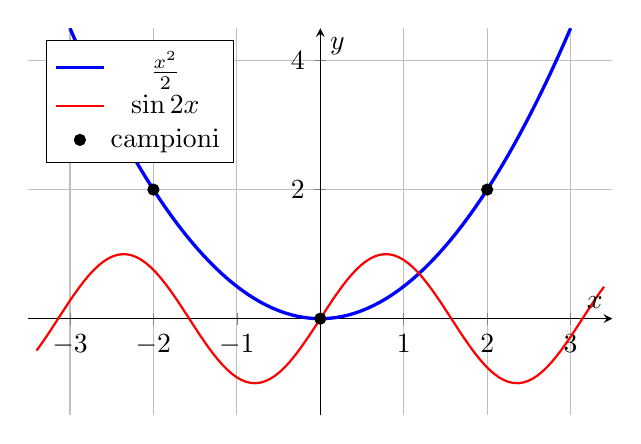
\begin{tikzpicture}
  \begin{axis}[
      axis lines=middle, xlabel=$x$, ylabel=$y$,
      xmin=-3.5, xmax=3.5, ymin=-1.5, ymax=4.5,
      grid=major, legend pos=north west,
      width=9cm, height=6.5cm]
    \addplot[blue, very thick, domain=-3:3, samples=80] {x^2/2};
    \addplot[red, thick, domain=-3.4:3.4, samples=120] {sin(deg(2*x))};
    \addplot[only marks, mark=*, black] coordinates {(-2,2) (0,0) (2,2)};
    \legend{$\frac{x^2}{2}$, $\sin 2x$, campioni}
  \end{axis}
\end{tikzpicture}
\end{document}
